\section{Accelerometer}

\subsection{Technology behind}
\label{sec:accl}
The accelerometer is a $3$-axis motion sensor. The sensor allows measuring acceleration of force in $m/s^2$ which are applied to a given device. The accelerometer can measure both roll, pitch, and yaw.

\begin{figure}[ht]
\begin{center}
 \label{fig:three-axis}
 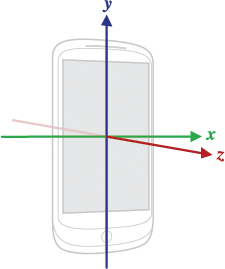
\includegraphics[scale=0.4]{img/axis_device.png}
\caption{A three-axis device}
\end{center}
\end{figure}

\subsection{Accelerometer in Android}
The accelerometer can be used by the Android platform in the following way. First a SensorManager is declared, this will handle the sensors on the platform.
After the initialization of the SensorManager, a Sensor of the type Accelerometer is declared.
The sensor base class contains different methods which we make use of when retrieving data from the accelerometer.

The main method we use is the onSensorChanged, which allows us to get accelerometer data each time the values of either of the three axis changes.

The accelerometer is accessed via a class, which extends the Service base class.
Here the accelerometer will be initialized and set up with the correct information.
After the initialization the accelerometer is ready to use, the user can call getAccelerometer() which will then start listening on the sensor to fire events when data change.

When either of the three axis change the onSensorChanged() will be fired. This will then retrieve the data from the accelerometer, and combine the three axis to a single value using the formula: $mAccelCurrent = sqrt(x^2 + y^2 + z^2)$. This makes sure the device can be placed in any orientation.

The data output is then analyzed to see if any movement is happening. The accelerometer is very precise to a dead-zone will have to be established.
An floating average of the $50$ last values from the accelerometer is calculated, giving a baseline for where the dead-zone is.
The system then calculates if a peak happens outside the dead-zone, and if so, the device is registered as moving.
If no peaks have been found for $50$ readings, the device is registered as not moving.

The moving state of the device will be sent to the server, along with the coordinates, and if the coordinates change a given distance and the moving state remains not moving, we assume that the user is not running or walking.\cite{androidsensor}\cite{androidaccl}

\subsection{Reflection}
A more in-depth analysis can be done in order to determine which kind of movement or activity the user is doing, but this would require a lot of data, and models of how different activities will appear as a graph.
This will both be very time consuming and heavy calculations for each user at any given time. The data from the accelerometer would also have to be run through a noise filter, as the values change a lot, even if the device is stationary.